\section{GraphQL}

GraphQL was developed by Facebook and refers to itself as the query language for an API. It provides the client with the opportunity to ask exactly for the data is needed. GraphQL offers the advantage that all data can be loaded from only one URL. With the help of the types within the GraphQL schema, the technology offers an understandable description of the
API for clients. \cite{misc:-:graphql-org} The functionality of GraphQL on the frontend can be compared to SQL on the database level. The client writes its queries with the desired fields from a dataset.

The official documentation states that GraphQL is a query language for APIs and a runtime for fulfilling those queries with your existing data. GraphQL provides a complete and understandable description of the data in your API, gives clients the power to ask for exactly what they need and nothing more, makes it easier to evolve APIs over time, and enables powerful developer tools. GraphQL is implemented in many languages and frameworks. It has a large ecosystem of libraries and tools.

\subsection{Origins and history}

GraphQL was initially developed at Facebook in 2012. In 2015 the project was made open-source and available to the public. The motivation behind the initial development of GraphQL was the limited flexibility of available API technologies like REST.

\subsection{GraphQL Characteristics}

Due 


\subsection{Apollo Server and Apollo Client}\label{subsection:background:graphql:apollo-server-client}

GraphQL has a specification and is a query language. Developing a GraphQL server and client is up to the application developer. Facebook has created its own GraphQL implementation of the specification in \ac{JS} with GraphQL.js for the backend and Relay for the frontend. Relay is a prominent example of a GraphQL client, but it is only available for Facebook's React framework. When evaluating different GraphQL clients, Apollo Client was chosen because it supports almost every possible programming language and framework.

\bigskip

\noindent Apollo Server is an open-source implementation of the GraphQL specification, and it offers any feature that the GraphQL specification states. Moreover, it supports Apollo Sandbox\footnote{\url{https://www.apollographql.com/docs/graphos/explorer/sandbox/}} out of the box. \cite{misc:-:background:graphql:apollo-server-introduction} Apollo Sandbox helps local development. Apollo Sandbox loads the GraphQL Schema from the server with the help of the Introspection Query. \cite{misc:-:background:graphql:apollo-sandbox} Such a development environment enables executing queries and mutations directly inside the browser.

\bigskip

\noindent Apollo Client is a community-driven project with npm packages for almost all frontend development environments like Angular, React, and Vue.js. The library fetches, caches, and manages the data of the application. The package for Angular is designed with Angular patterns in mind to integrate perfectly with the framework. Apollo Client offers the possibility to cache already made requests. \cite{misc:-:background:graphql:apollo-angular-client-overview} \cite{misc:-:background:graphql:apollo-client-overview} Caching is especially important as it can reduce the number of roundtrips to the server. The inner workings of the cache to prove or disprove the first hypothesis are explained in the following sections.

\subsubsection{How does the in-memory cache work?}\label{subsubsection:background:graphql:apollo-server-client:in-memory-cache-working}

This section describes how the caching mechanism of the Apollo Client works. The structure of the cache is a local, normalized, in-memory cache. All GraphQL requests made with Apollo Client are cached inside the browser's memory by default. The cache enables Apollo Client to respond almost immediately to queries for already-cached data without sending a network request. This mechanism is needed to reduce round-trips to the server in subsequent requests of the same query because the requested data can be served from the cache. \cite{misc:-:background:graphql:apollo-client-cache-overview} Caching mechanisms generally reduce the server's load but introduce issues with cache management.

\bigskip

\noindent \textbf{Apollo Client} includes a caching interface called \texttt{ApolloCache} and a proprietary implementation named \texttt{InMemoryCache}. Several Open-Source alternatives implement the \texttt{ApolloCache} interface, but Apollo's implementation is well-supported and receives regular updates.

\bigskip

\noindent Figure~\ref{fig:background:graphql:user-query-first-time} shows an exemplary query to fetch a user with its unique id. First, the Apollo Client checks whether the user with the given id is already stored inside the cache. If the query with that id has yet to be executed, a network query to fetch the user must be made. The result from the GraphQL Server is stored inside the cache and returned to the application. Four steps must be made to render data on the screen. \cite{misc:-:background:graphql:apollo-client-cache-overview}

\ifshowImages
\begin{figure}[H]
  \centering
  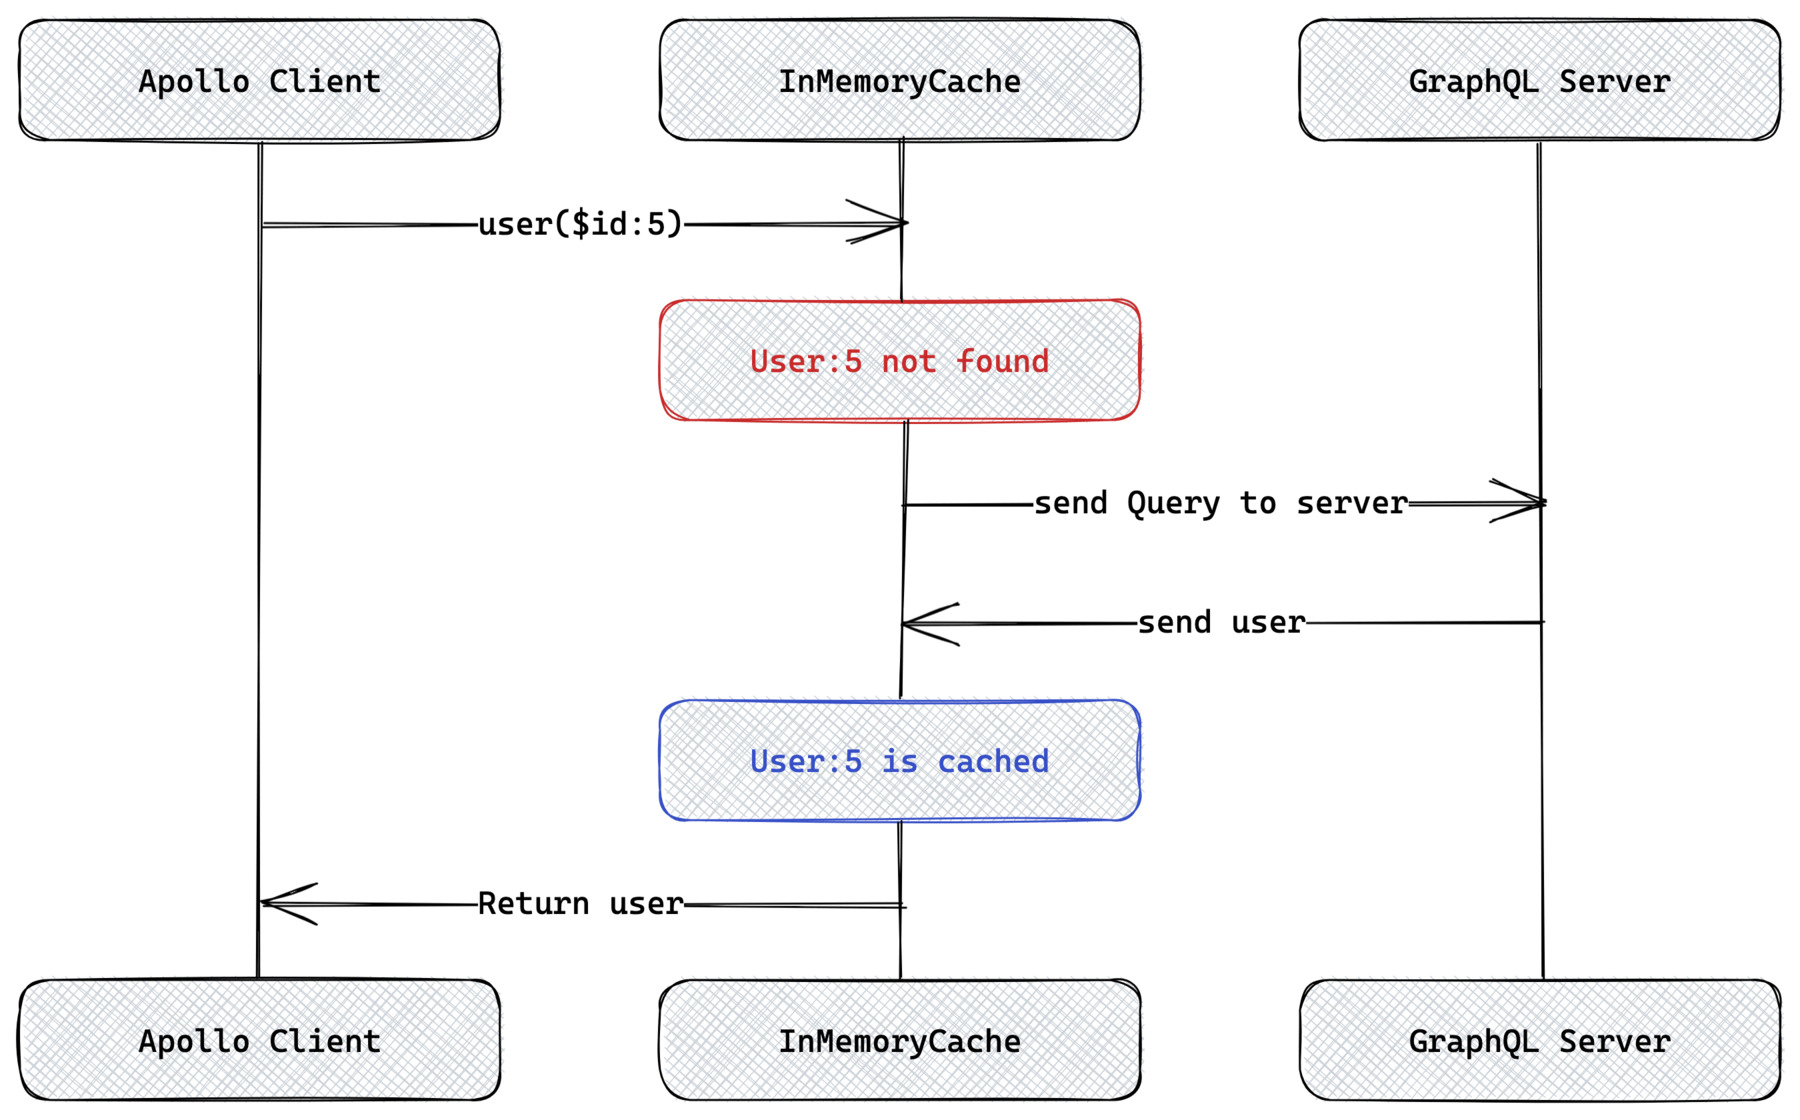
\includegraphics[width=0.6\linewidth]{images/background/graphql/apollo/apollo-client-basic-cache.jpg}
  \caption{The execution of a GraphQL query that is not stored in the cache. (Adapted from \cite{misc:-:background:graphql:apollo-client-cache-overview})}\label{fig:background:graphql:user-query-first-time}
\end{figure}
\fi

\noindent If a request with the same user id is made again, the flow of execution looks like in Figure \ref{fig:background:graphql:user-query-second-time}. As seen in the figure, no network request has to be made to the GraphQL \ac{API}, because everything is served from the Apollo Cache alone. Compared to the four steps in Figure \ref{fig:background:graphql:user-query-first-time}, only two steps need to be done here. \cite{misc:-:background:graphql:apollo-client-cache-overview}

\ifshowImages
\begin{figure}[H]
  \centering
  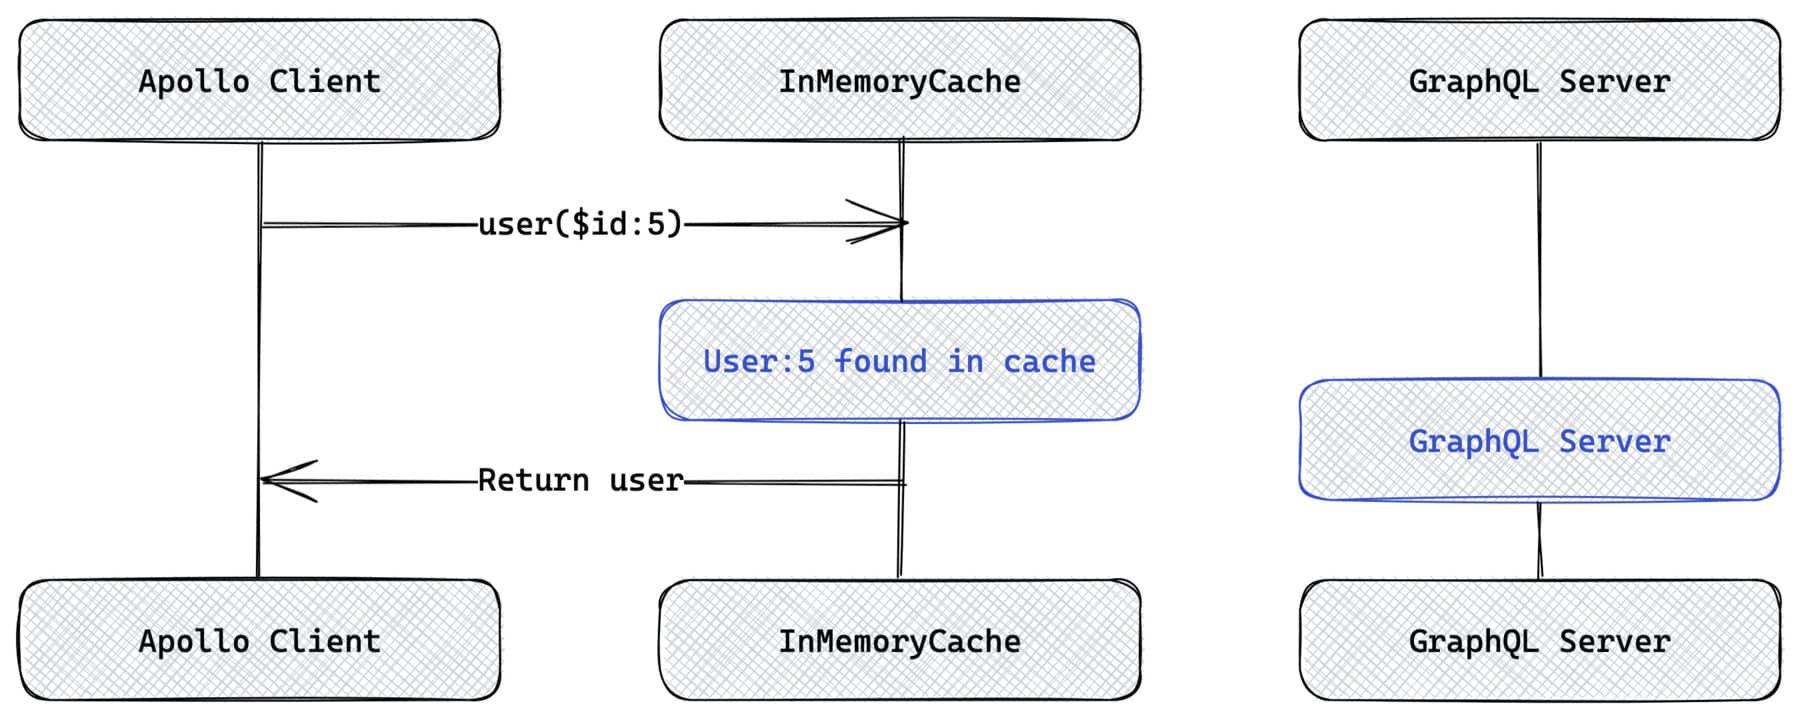
\includegraphics[width=0.7\linewidth]{images/background/graphql/apollo/apollo-client-basic-cache-warm.jpg}
  \caption{Execute the same query, which reduces the necessary steps. (Adapted from \cite{misc:-:background:graphql:apollo-client-cache-overview})}\label{fig:background:graphql:user-query-second-time}
\end{figure}
\fi

\subsubsection{Data normalization}\label{subsubsection:background:graphql:apollo-server-client:data-normalization}

Whenever the Apollo Client receives the response data of a query, it does the following. To correctly understand cache updates, it is essential to the structure of the cache before. The \texttt{InMemoryCache} is a simple normalized \ac{JS} object. The Apollo Client stores the data as a flat lookup table of objects referencing each other. An empty cache is just an empty object. These objects correspond to the objects that are returned by GraphQL queries. A single cache object might include fields fetched by multiple queries, allowing multiple queries to fetch different fields for the same object. \cite{misc:-:background:graphql:apollo-client-cache-overview} The following paragraphs describe the steps from a GraphQL query to the objects inside the cache.

\paragraph{1. Identify objects}\label{paragraph:background:graphql:apollo-server-client:data-normalization:identify-objects}

The cache identifies all distinct objects included in the query response. For example, take the query from Listing \ref{code:background:graphql:query-user-cache}, which returns the \texttt{id}, \texttt{username}, and \texttt{email} of every user.

\ifshowListings
\begin{listing}[H]
  \begin{minted}{typescript}
query {
  users {
    id
    username
    email
  }
}
  \end{minted}
  \caption{GraphQL query that fetches the id, username, and email of every user.}\label{code:background:graphql:query-user-cache}
\end{listing}
\fi

\noindent The server responds with the following response seen in Listing \ref{code:background:graphql:query-user-response-result}. The \texttt{\_\_typename} property is automatically appended to the query by the Apollo Client to identify the object.

\ifshowListings
\begin{listing}[H]
  \begin{minted}{typescript}
{
  users: [
    {
      __typename: 'User',
      id: '36bad921-8fcf-4f33-9f29-0d3cd70205c8',
      username: 'Florian',
      email: 'florian@test.io'
    },
    {
      __typename: 'User',
      id: 'a2096556-9a4e-4994-9de8-86c9e85ed6a1',
      username: 'Lisa',
      email: 'lisa@test.io'
    }
  ]
}
  \end{minted}
  \caption{The result of the GraphQL query from Listing \ref{code:background:graphql:query-user-cache}.}\label{code:background:graphql:query-user-response-result}
\end{listing}
\fi

The caching mechanism identifies the following objects to be cached.

\begin{itemize}
  \item A \texttt{User} with id \texttt{36bad921-8fcf-4f33-9f29-0d3cd70205c8}
  \item A \texttt{User} with id \texttt{a2096556-9a4e-4994-9de8-86c9e85ed6a1}
\end{itemize}

\paragraph{2. Generate cache IDs}\label{paragraph:background:graphql:apollo-server-client:data-normalization:generate-cache-ids}

After identifying all objects, the cache generates a cache ID for each object. A cache ID uniquely identifies a particular object while it is in the \texttt{InMemoryCache}.

\noindent So, the cache IDs for the objects from the previous section are:

\begin{itemize}
    \item \texttt{User:36bad921-8fcf-4f33-9f29-0d3cd70205c8}
    \item \texttt{User:a2096556-9a4e-4994-9de8-86c9e85ed6a1}
\end{itemize}

\noindent By default, an object's cache ID is concatenated with the object's \texttt{\_\_typename} and \texttt{id} (or \texttt{\_id}) fields. If the cache cannot generate a cache ID for a particular object, that object is directly stored inside its parent object and must be referenced via the parent. Therefore the cache is not always completely flat. This behavior is shown with the query in Listing \ref{code:background:graphql:no-id-query-user-cache}. 

\ifshowListings
\begin{listing}[H]
  \begin{minted}{typescript}
query {
  allUsers {
    id
    username
    Title {
      name
    }
  }
}
  \end{minted}
  \caption{Fetch the \texttt{id}, \texttt{username} and the \texttt{name} of the title of the user, without the \texttt{id} of the title.}\label{code:background:graphql:no-id-query-user-cache}
\end{listing}
\fi

\noindent The query from the listing misses the \texttt{id} field inside the Title field. Therefore the cache stores the Title object directly inside the user object. The result inside the cache is shown in the listing
\ref{code:background:graphql:no-id-query-user-cache-representation}. 

\ifshowListings
\begin{listing}[H]
  \begin{minted}{typescript}
{
  'User:36bad921-8fcf-4f33-9f29-0d3cd70205c8': {
    __typeName: 'User',
    id: '36bad921-8fcf-4f33-9f29-0d3cd70205c8',
    username: 'Florian',
    Title: { name: 'BSc.' }
  },
  'User:a2096556-9a4e-4994-9de8-86c9e85ed6a1': {
    __typeName: 'User',
    id: 'a2096556-9a4e-4994-9de8-86c9e85ed6a1',
    username: 'Lisa',
    Title: { name: 'BSc.' }
  }
}
  \end{minted}
  \caption{The content of the cache after fetching the query from Listing \ref{code:background:graphql:no-id-query-user-cache}.}\label{code:background:graphql:no-id-query-user-cache-representation}
\end{listing}
\fi

\noindent Omitting IDs from a query should be avoided. If data of an un-normalized object has to be updated, every occurrence of the item in the cache has to be updated manually. It should be avoided that the same thing is queried, sometimes with an id and sometimes without, because Apollo Client will throw an error when trying to update the cache after such a query.

\paragraph{3. Replace object fields with references}\label{paragraph:background:graphql:apollo-server-client:data-normalization:replace-object-fields-with-references}

Next, the cache takes each field that contains an object and replaces its value with a reference to the appropriate object. Listing \ref{code:background:graphql:nested-query-user-cache} shows a query that demonstrates how the objects from a query are transformed in the \texttt{InMemoryCache} representation.

\ifshowListings
\begin{listing}[H]
  \begin{minted}{typescript}
query {
  allUsers {
    id
    username
    Title {
      id
      name
    }
  }
}
  \end{minted}
  \caption{A GraphQL query to fetch all users.}\label{code:background:graphql:nested-query-user-cache}
\end{listing}
\fi

Listing \ref{code:background:graphql:nested-query-response-user-cache} shows a single result from the GraphQL server for the query from Listing \ref{code:background:graphql:nested-query-user-cache}.

\ifshowListings
\begin{listing}[H]
    \begin{minted}{typescript}
{
  __typename: 'User',
  id: '36bad921-8fcf-4f33-9f29-0d3cd70205c8',
  username: 'Florian',
  title: {
    __typename: 'Title',
    id: '2adb1120-d911-4196-ab1b-d5043cc7a00a',
    name: 'BSc.'
  }
}
    \end{minted}
    \caption{The result of the GraphQL query from Listing \ref{code:background:graphql:nested-query-user-cache}.} \label{code:background:graphql:nested-query-response-user-cache}
\end{listing}
\fi

\noindent And Listing \ref{code:background:graphql:nested-query-response-after-replacement} shows how the object is stored inside the \texttt{InMemoryCache}.

\ifshowListings
\begin{listing}[H]
  \begin{minted}{typescript}
{
  __typename: 'User',
  id: '36bad921-8fcf-4f33-9f29-0d3cd70205c8',
  username: 'Florian',
  title: { __ref: 'Title:36bad921-8fcf-4f33-9f29-0d3cd70205c8' }
}
  \end{minted}
  \caption{The structure of the cache after the user object is stored.}\label{code:background:graphql:nested-query-response-after-replacement}
\end{listing}
\fi

\noindent The \texttt{title} field now references the appropriate normalized \texttt{Title} object. If another \texttt{User} with the same \texttt{title} is stored inside the in-memory cache, that normalized \texttt{Title} object is reused. Normalization can drastically reduce data duplication inside the cache, and it also helps to make the data stay synchronous with the server.

\paragraph{4. Store normalized objects}\label{paragraph:background:graphql:apollo-server-client:data-normalization:store-normalized-objects}

The resulting objects are stored inside the cache's flat lookup table. Whenever an incoming object has the same cache ID as an existing cached object, the fields of those objects are merged. If the incoming and the existing object share existing fields, the incoming object overwrites the cached value for those fields. Fields that exist in only one object are preserved. This normalization constructs a partial copy of the graph on our client. \cite{misc:-:background:graphql:apollo-client-cache-overview}

\bigskip

\noindent Listing \ref{code:background:graphql:nested-query-user-cache-representation} shows how normalized objects are stored. Each user contains a reference to a title. Both users have the same title. Therefore the server returned duplicate data. However, the cache normalization causes the title to be only present once inside the cache. This behavior is constructive because when a cache item is updated, the entire cache object does not have to be traversed in search of the instance that has been changed. Only a single item has to be updated. The cache normalization works when the query contains either a \texttt{\_id} or \texttt{id} field.

\ifshowListings
\begin{listing}[H]
    \begin{minted}{typescript}
{
  'User:36bad921-8fcf-4f33-9f29-0d3cd70205c8': {
    __typeName: 'User',
    id: '36bad921-8fcf-4f33-9f29-0d3cd70205c8',
    username: 'Florian',
    Title: { __ref: 'Title:2adb1120-d911-4196-ab1b-d5043cc7a00a' },
  },
  'User:a2096556-9a4e-4994-9de8-86c9e85ed6a1': {
    __typeName: 'User',
    id: 'a2096556-9a4e-4994-9de8-86c9e85ed6a1',
    username: 'Lisa',
    Title: { __ref: 'Title:2adb1120-d911-4196-ab1b-d5043cc7a00a' },
  }
  'Title:2adb1120-d911-4196-ab1b-d5043cc7a00a': {
    __typeName: 'Title',
    id: '2adb1120-d911-4196-ab1b-d5043cc7a00a',
    name: 'BSc.',
  },
}
  \end{minted}
  \caption{The structure of the cache with the result from the query from Listing \ref{code:background:graphql:nested-query-user-cache}.}\label{code:background:graphql:nested-query-user-cache-representation}
\end{listing}
\fi

\subsubsection{Understanding the structure of the cache}\label{subsubsection:background:graphql:apollo-server-client:understanding-cache-structure}

Apollo Client offers development tools for the browser in the form of browser extensions. The Apollo Client Developer Tools\footnote{\url{https://chrome.google.com/webstore/detail/apollo-client-devtools/jdkknkkbebbapilgoeccciglkfbmbnfm}} can be installed for Chrome and Firefox. The extension can be found in the Chrome Web Store and the Firefox Add-ons Store. The browser extension adds a tab to the browser inspection tools. \cite{misc:-:background:graphql:apollo-developer-tools} The view of the cache contents from the Apollo Client Development Tools can be seen in Figure \ref{fig:background:graphql:apollo:apollo-dev-tools}.

\ifshowImages
  \begin{figure}[H]
    \centering
    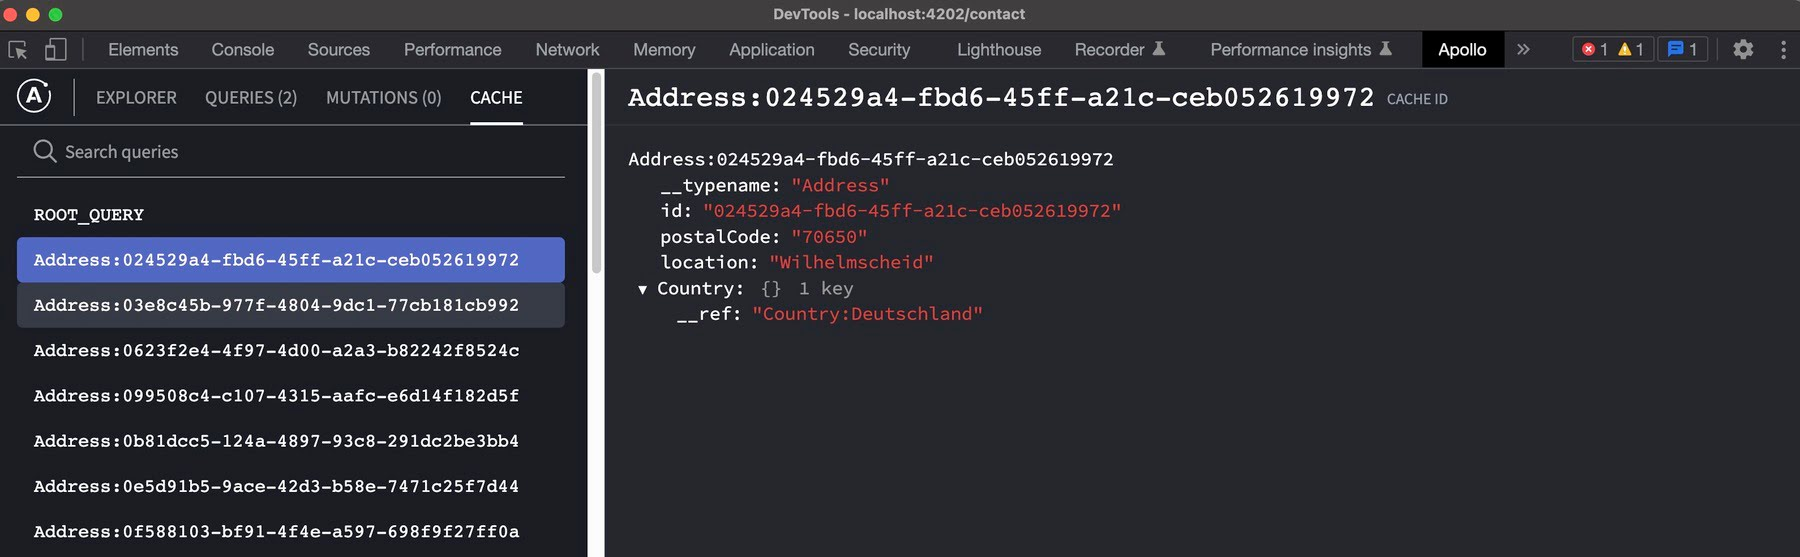
\includegraphics[width=1\linewidth]{images/background/graphql/apollo/apollo-dev-tools.jpg}
    \caption{The content of the cache inside the Apollo Client Developer Tools.}\label{fig:background:graphql:apollo:apollo-dev-tools}
  \end{figure}
\fi

\noindent The development tools offer the following four main features: \cite{misc:-:background:graphql:apollo-developer-tools}

\begin{itemize}
  \item \textbf{GraphiQL}: Send queries to the server through the web application's configured Apollo Client instance, or query the Apollo Client cache to see what data is loaded.
  \item \textbf{Watched query inspector}: View active queries, variables, cached results, and re-run individual queries.
  \item \textbf{Mutation inspector}: View active mutations and their variables, and re-run individual mutations.
  \item \textbf{Cache inspector}: Visualize the Apollo Client and search it by field name and/or value.
\end{itemize}

\noindent Another method to access the content of the cache is through the \texttt{window} object in \ac{JS}. The object can be accessed through \texttt{window.\_\_APOLLO\_CLIENT\_\_.cache.extract()} inside the browser's development tools. The result of this method invocation can be seen in Figure \ref{fig:background:graphql:apollo:apollo-cache-browser-window}.

\ifshowImages
  \begin{figure}[H]
    \centering
    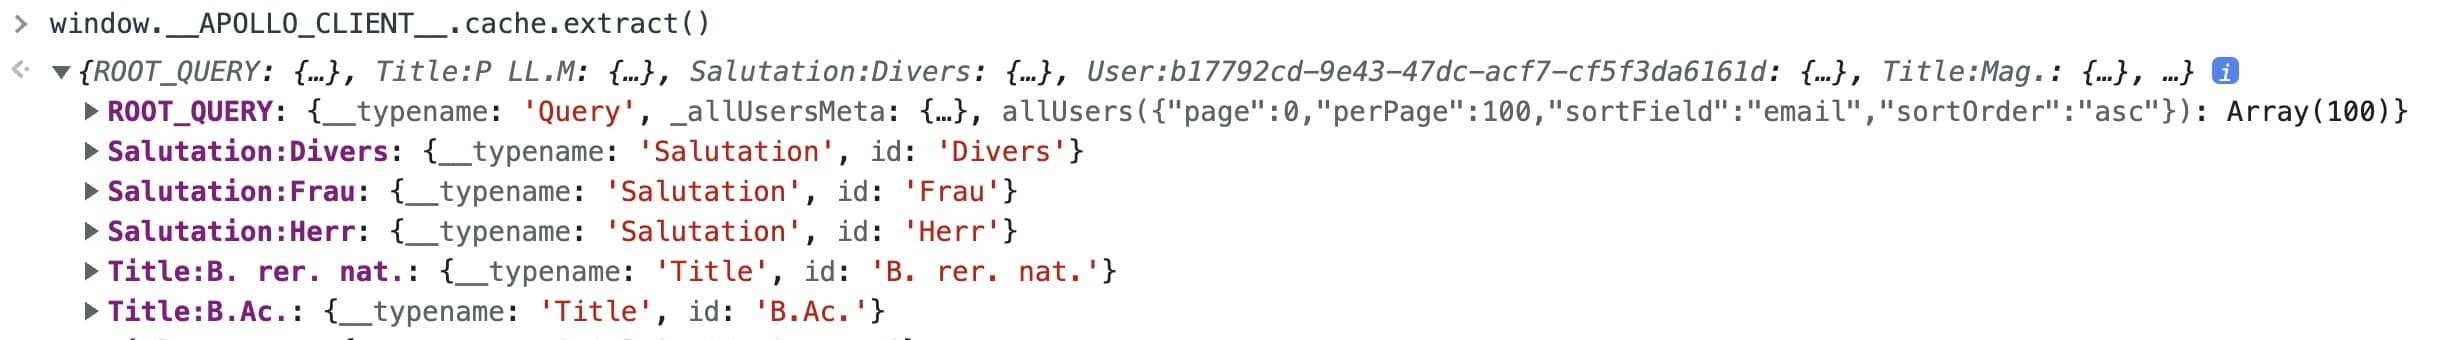
\includegraphics[width=1\linewidth]{images/background/graphql/apollo/apollo-cache-browser-window.jpg}
    \caption{View the content of the cache inside the development tools.}\label{fig:background:graphql:apollo:apollo-cache-browser-window}
  \end{figure}
\fi

\noindent With this approach, the content of the cache can be explored with the help of \ac{JS} methods inside the browser development tools.

\subsubsection{Type-Policies}\label{subsubsection:background:graphql:apollo-server-client:type-policies}

Type policies are a way to define how the client stores and manages data in the cache. The constructor of the \texttt{InMemoryCache} accepts type policies as an object. The \texttt{typePolicies} object the behavior of the cache can be customized on a type-by-type basis. Type policies are fine-grained; they allow to customize how a specific field inside the cache is read and written. A type policy contains multiple field policies that customize the behavior of the fields for that type. \cite{misc:-:background:graphql:apollo-client-cache-reading-writing}

\bigskip

\noindent A field policy for a field consists of: \cite{misc:-:background:graphql:apollo-client-cache-reading-writing}

\begin{itemize}
  \item A \texttt{read} function which is called when the field is read from the cache.
  \item A \texttt{merge} function which is called when the field is written to the cache.
  \item An array of fields, which are the key arguments that identify an object. This so-called \texttt{keyArgs} avoids storing duplicate data in the cache.
\end{itemize}

\paragraph{Read function}

Listing \ref{code:background:graphql:read-type-policy} shows the definition of a \texttt{read} function. The cache calls that function when the client queries for a user's first name. The \texttt{InMemoryCache} then returns the function's response instead of the cached value. The first parameter of the function is the current value of the field. The second parameter is an object that contains the arguments of the field and several helper functions and properties. \cite{misc:-:background:graphql:apollo-client-cache-reading-writing} The \texttt{read} function of Listing \ref{code:background:graphql:read-type-policy} returns a default value for the \texttt{firstName} of the \texttt{User} type when a value is unavailable in the cache. If a value exists in the cache, the value is returned unmodified.

\ifshowListings
\begin{listing}[H]
    \begin{minted}{typescript}
new InMemoryCache({
  typePolicies: { User: { fields: {
    firstName: {
      read(value, options) {
        return value ?? 'Unknown';
      }
    }
  }}}
});
    \end{minted}
    \caption{Provide a default value for the  \texttt{firstName} field.}\label{code:background:graphql:read-type-policy}
\end{listing}
\fi

\paragraph{Merge function}

The \texttt{merge} function for a field is called whenever the field is about to be written with an incoming value. The field's new value is set to the \texttt{merge} function's return value instead of the original value.  An everyday use case for the \texttt{merge} function is to define a field policy for a field that holds an array. By default, the existing collection is completely replaced by the incoming array. However, sometimes, both arrays should be concatenated. This pattern is used with paginated lists, where the incoming page should be merged with the existing pages. The parameters are the current value, the incoming value, and the options, just like in the \texttt{read} function. \cite{misc:-:background:graphql:apollo-client-cache-reading-writing}

\bigskip

\noindent Listing \ref{code:background:graphql:write-type-policy} shows the definition of a \texttt{merge} function. Whenever a new transaction for the bank account is fetched, the existing and the incoming transactions are merged. Initially, \texttt{existing} is undefined; therefore, \texttt{existing} is assigned a default parameter.

\ifshowListings
\begin{listing}[H]
    \begin{minted}{typescript}
new InMemoryCache({
  typePolicies: { BankAccount: { fields: {
    transaction: {
      merge(existing = [], incoming: unknown[], options) {
        return [...existing, ...incoming];
      },
    },
  }}},
});
    \end{minted}
    \caption{Merge the existing and incoming transactions in a \texttt{merge} function.}\label{code:background:graphql:write-type-policy}
\end{listing}
\fi
